\chapter{Methodology and Architecture} \label{Methodology}

\section{Introduction}

This chapter describes the methodologies for the developed payloads and the defence against them. It will start with the attacker's point of view, examine existing attacks in the context of the MITRE ATT\&CK framework, introduce new attacks and then move on to the defence system.


\section{The MITRE ATT\&CK Framework}

ATT\&CK~\cite{MITREATTCK} is an openly accessible knowledge base of adversary tactics and techniques developed by the security advisor firm MITRE~\cite{WhoWeAre}. It can be used for threat modelling and as a general overview of different types of cyber-attacks.
It features 14 attack categories subdivided into 8-43 techniques. One example is the category Reconnaissance which is subdivided into Active Scanning, Gather Victim Host Information, Gather Victim Identity Information, Gather Victim Network Information, Gather Victim Org Information, Phishing for Information, Search Closed Sources, Search Open Technical Databases, Search Open Websites/Domains and Search Victim Owned Websites.



\subsection{Evaluation of Existing Attack Scripts}

This thesis will explore several of these categories and techniques and assess whether a script for each category is available in the official O.MG Payloads GitHub repository \cite{Hak5Omgpayloads2024}. \\
It is important to note that the most basic attack that can be executed via Keyboard Injection is also the most versatile and one of the most dangerous ones. It is a simple script that downloads any malware, which as a result, could execute any software-based attack.
This analysis will therefore focus on implementations solely based on keyboard injection and will not feature payloads that include downloading additional malware.
The thesis will not examine all 14 categories and instead highlight the most relevant ones.

\subsubsection{Reconnaissance}

Reconnaissance involves actively or passively gathering information. The gathered information can be used to inform the preparations
for a bigger attack or to further additional reconnaissance efforts. This category includes scanning network traffic and gathering host information such as name, Internet Protocol (IP) address, operating system,
hardware information, credentials, email, or information about a network. Phishing also belongs into this category, as does the purchase of information about the system from legal or illegal data brokers or gathering publicly available information, for example from the Internet \cite{MITREATTCK}.

This is a field in which keyboard injection can cause considerable damage. There exist many exfiltration scripts, that download sensitive files, exfiltrate passwords, gather network and device information, or social engineer the user to enter sensitive data on malicious sites.
For example, \verb|Harvester_OF_SORROW| \cite{OmgpayloadsPayloadsLibrary} exfiltrates login information from Firefox on Windows 10. Other examples for password extraction are \verb|SudoSnatch| \cite{OmgpayloadsPayloadsLibrary} which exfiltrates sudo passwords, and \verb|WLAN-Windows-Passwords| \cite{OmgpayloadsPayloadsLibrary} which steals WLAN passwords and sends them to the attacker via a Discord webhook. 
\verb|OMGLogger| \cite{OmgpayloadsPayloadsLibrary} which leverages the logging capabilities of the O.MG cable and sends the keystrokes live to the attacker's server. \\
The collection on GitHub contains a folder dedicated to exfiltration scripts, that can find data on a network, a printer, a target's Spotify, PowerShell history, log files, MySQL history,
Firefox browser cookies, photos, or send periodic screenshots. \\
Similarly, there is a folder with scripts on phishing  \cite{OmgpayloadsPayloadsLibrary}, however, it is less extensive. The three payloads build on the idea of faking a pop-up,
where the user is prompted to (re)submit login data. Each of the existing phishing scripts has software prerequisites and is written for Linux. \\


\subsubsection{Resource Development}

Resource Development is what a malicious actor does when they want to establish resources that can help them mount an attack, such as getting access to specific email addresses,
system accounts, or target systems. It also includes setting up servers or bots that could be used for an attack or creating and cultivating accounts to build a persona \cite{MITREATTCK}.\\
Resource Development is an important part of injection attacks in conjunction with data exfiltration. This is apparent in payloads like
\verb|ExfiltrateLinuxLogFiles| \cite{OmgpayloadsPayloadsLibrary}, \verb|WLAN-Windows-Passwords| \cite{OmgpayloadsPayloadsLibrary}, \verb|-OMG-Credz-Plz|
\cite{OmgpayloadsPayloadsLibrary}, or \verb|OMG-AwarenessTraining| \cite{OmgpayloadsPayloadsLibrary} which send the exfiltrated data to a private server, Discord webhook, or Dropbox.
Any data transmission from the O.MG cable to the attacker will require communication resources and, therefore, some degree of resource development.


\subsubsection{Initial Access}

Initial Access is about an adversary trying to get access to a target network\cite{MITREATTCK}. Some examples of how this can be done with keyboard injection are
\verb|revshell_windows| and \verb|win_winrm-backdoor| \cite{OmgpayloadsPayloadsLibrary}; payloads that establish remote control over a targeted computer.
Through that access point, the network can be infiltrated. Similarly, passwords for networks can be exfiltrated from a target computer using \verb|WLAN-Windows-Passwords|
\cite{OmgpayloadsPayloadsLibrary}. Knowing the passwords makes gaining initial access a lot easier. \\

\subsubsection{Execution}

Execution includes all techniques used to run malicious code on a target's computer or server, whether through shells, coding environments, hotkeys, native APIs, or by relying on the user to trigger code execution, such as clicking on a link or file \cite{MITREATTCK}. 
Running malicious code is at the core of Keyboard Injection attacks. It is their alpha and omega and can be found in every script of the collection.

\subsubsection{Persistence} \label{persistence}

Persistence stresses the longevity and robustness of an attack over time. To this end, accounts and access rights can be manipulated, SAM keys stolen or modified, new devices registered for two-factor authentication, system processes created or modified  (i.e. modifying PowerShell profile scripts), and much more. This can be achieved by using external remote services, or manipulating pre-OS boot mechanisms \cite{MITREATTCK}. \\
An example of this kind of technique is the remote access that can be gained by scripts like \verb|revshell_macOS| \cite{OmgpayloadsPayloadsLibrary}
or remote control access establishment as demonstrated by \cite{bojovicRisingThreatHardware2019}. \\
This category also includes attack scheduling, which can easily be achieved by DuckyScript, using the `DELAY` command, the remote trigger, or the Geofencing feature \cite{hak5MGCable}.

\subsubsection{Privilege Escalation}

Privilege Escalation includes techniques used to gain higher-level permissions in a network or system by bypassing account controls, abusing elevation control mechanisms, accessing or stealing tokens, account manipulation, or breaking out of containers to gain access to a host \cite{MITREATTCK}. \\
Account manipulation can easily be achieved with the correct recon. Especially if the login credentials of an administrator can be logged (for example with \verb|OMGLogger| \cite{OmgpayloadsPayloadsLibrary}) or are stored somewhere in the system, where they can be exfiltrated using payloads such as \verb|SudoSnatch| \cite{OmgpayloadsPayloadsLibrary} or \verb|Everything-Password-Stealer| \cite{OmgpayloadsPayloadsLibrary}.

\subsubsection{Credential Access}

Credential Access involves adversaries attempting to steal usernames and passwords, a technique commonly implemented by existing GitHub scripts as discussed in previous sections.
Examples are \verb|SudoSnatch| \cite{OmgpayloadsPayloadsLibrary}, \verb|Everything-Password-Stealer| \cite{OmgpayloadsPayloadsLibrary}, or this paper using a BadUSB:  \cite{muslimImplementationAnalysisUSB2020}.


\subsubsection{Collection}
After a target has been infiltrated, the data collection process can start. It consists of techniques like Man-in-the-Middle (MITM), compressing data, browser session hijacking, audio and or image capture, clipboard data exfiltration, email collection, keylogging, etc. \cite{MITREATTCK}. \\
Keylogging specifically is one of the features of the O.MG cable, as discussed previously, and further extended by \verb|Persistent_Keylogger-Telegram_Based|
\cite{OmgpayloadsPayloadsLibrary}. Image capturing is demonstrated by \verb|Screen-Shock| \cite{OmgpayloadsPayloadsLibrary}, and the theft of photos by \\  \verb|ExfiltratePhotosThroughShell| \cite{OmgpayloadsPayloadsLibrary}.


\subsubsection{Exfiltration}

Exfiltration focuses on the methods used to transmit stolen data to the attacker \cite{MITREATTCK}. As discussed in the section about Data Reconnaissance, exfiltration can happen in various ways. The examples from the GitHub repository include sending the data to (Discord) webhooks or a
Dropbox. Some examples for this are:  \verb|ExfiltrateLinuxLogFiles|, \verb|WLAN-Windows-Passwords|, \verb|-OMG-Credz-Plz|, or \verb|OMG-AwarenessTraining|  \cite{OmgpayloadsPayloadsLibrary}.

\subsubsection{Impact}

The techniques in the category Impact are not widely represented in the GitHub repository. They include scripts that try to manipulate, interrupt or destroy systems and data \cite{MITREATTCK}.
However, it has been shown by \cite{lawalFacilitatingCyberenabledFraud2022} that it is possible to change, meaning manipulate, data on a target's
computer without leaving traces of an attack, thereby framing the computer's user(s) for the data change. It has therefore been shown to be possible to use the O.MG cable for Impact.

\subsection{Conclusions drawn from existing Payloads}

From the examples above it is apparent, that a wide variety of attacks and techniques are available with DuckyScript and a malicious USB device. Many sections of the ATT\&CK model play a role and are part of various scripts for the O.MG cable that already exist. The most prevalent ATT\&CK categories from the available code base are focused on the collection and exfiltration of data and the infiltration of systems and networks. The ``impact'' category is scarcely covered by existing payloads, suggesting significant room for development in this area.
Differences in coverage might be explained through the nature of the attack type; for some attacks, it is simply not effective to use keyboard injection. Take for example ``Supply Chain Compromise'' (ID T1195) \cite{SupplyChainCompromise} which describes supply chain attacks for which products are manipulated before their usage. Although it would theoretically be possible to manipulate, for example, firmware of a computer chip, there may be much more effective vectors than a keyboard injection attack; it simply requires too much very detailed intelligence. Attacks for which the O.MG cable is more useful, like simple attacks utilizing PowerShell commands, or pranks like playing a video, sounds, or changing background pictures are more common. 
Another aspect to consider is that this repository is not designed to comply with the MITRE ATT\&CK framework and has only 36 contributors. Open-source programmers may create payloads for topics that interest them or align with their expertise. Their goal is not to cover as many attacks as possible. One last consideration concerning the payloads in the repository is content moderation. It is possible that some payloads are not tolerated on the repository. However, this theory is unlikely since the entire premise of Hak5 is to make the dangers and attacks of the black hat world as widely known as possible to be able to defend against them.\\  
In line with this sentiment, this thesis will develop novel payloads in the following chapters. Splitting the enormous spectrum of all possible cyber attacks into only 14 categories means that each of those categories still covers a large section of attack types, each of which in turn can have a multitude of aspects and implementations. For this reason, the payloads developed in this thesis cannot be exclusively attributed to ``Impact`'' or other underrepresented categories. Instead, they represent a collection of novel payloads associated with subtechniques from various categories. Each payload is inspired by a specific subtechnique and has not yet been included in the O.MG Payloads GitHub repository. These are realistic attacks where HID injection is possible, representing only a small selection of potential payloads still 'missing' from the repository.

\newpage
\section{Payload Architecture}


This section will give an overview of the methodologies of the developed payloads and defences. Their implementations will be discussed in the next Section \ref{Implementation}. \\


\subsection{Setup for an HID Injection Attack}

When preparing for an HID injection attack, a malicious actor has to pay attention to the following 5 points:

\begin{enumerate}
    \item Target
    \item Circumstance
    \item Required Hardware
    \item Required Software
    \item Place and Timing
\end{enumerate}


The target is the most crucial element and specifically for injection attacks it is much more important \emph{what} the target is instead of who. The answer to this question determines which kind of attack is carried out and what the basic payload is. The question of \emph{who} is important in so far as it influences the next point: Circumstance. For example, a target that always locks their computer when stepping away from it creates the circumstance of a locked screen, in which case a password must be acquired and injected first. A circumstance is also the target's operating system, all the information about their hardware, the defence software that might be in place, and other behavioural information on the target, for example, their habits. Once these two factors have been sufficiently explored, the question of hardware comes up. What should be used? In some specific situations, a USB stick might be best. This could, for example, be the case when the attacker has access to a target's workstation and can place the stick in an envelope with the target's name on it to trick them into plugging it in. In other situations, it might be ideal to modify a keyboard and build the malicious hardware into it, or to alter a charging port in a public space. For many stealthy situations, the O.MG cable can be perfect because it seems so harmless. With a clear goal, enough information about the target's circumstance and the hardware question decided, the payload may be developed. While a basic script might already exist, it likely has to be modified to fit the specific situation. For example, it will need adjustments if it includes commands that require administrative rights or absolute file paths, or it might profit from adapting delays depending on the speed of the target's machine. \\
Once the setup is complete, the payload has to be injected at the right time and place. The O.MG cable's remote trigger and geofencing features come in handy for this purpose. To avoid detection of and interference with the payload it is best to execute it when no one is watching or in such a fast fashion that it is over before it is noticed.\\
Naturally, these steps influence each other or may overlap. Figure \ref{Flow Diagram Development process payload} serves as a visualization of the process:


\begin{figure}[H]
    \centering
    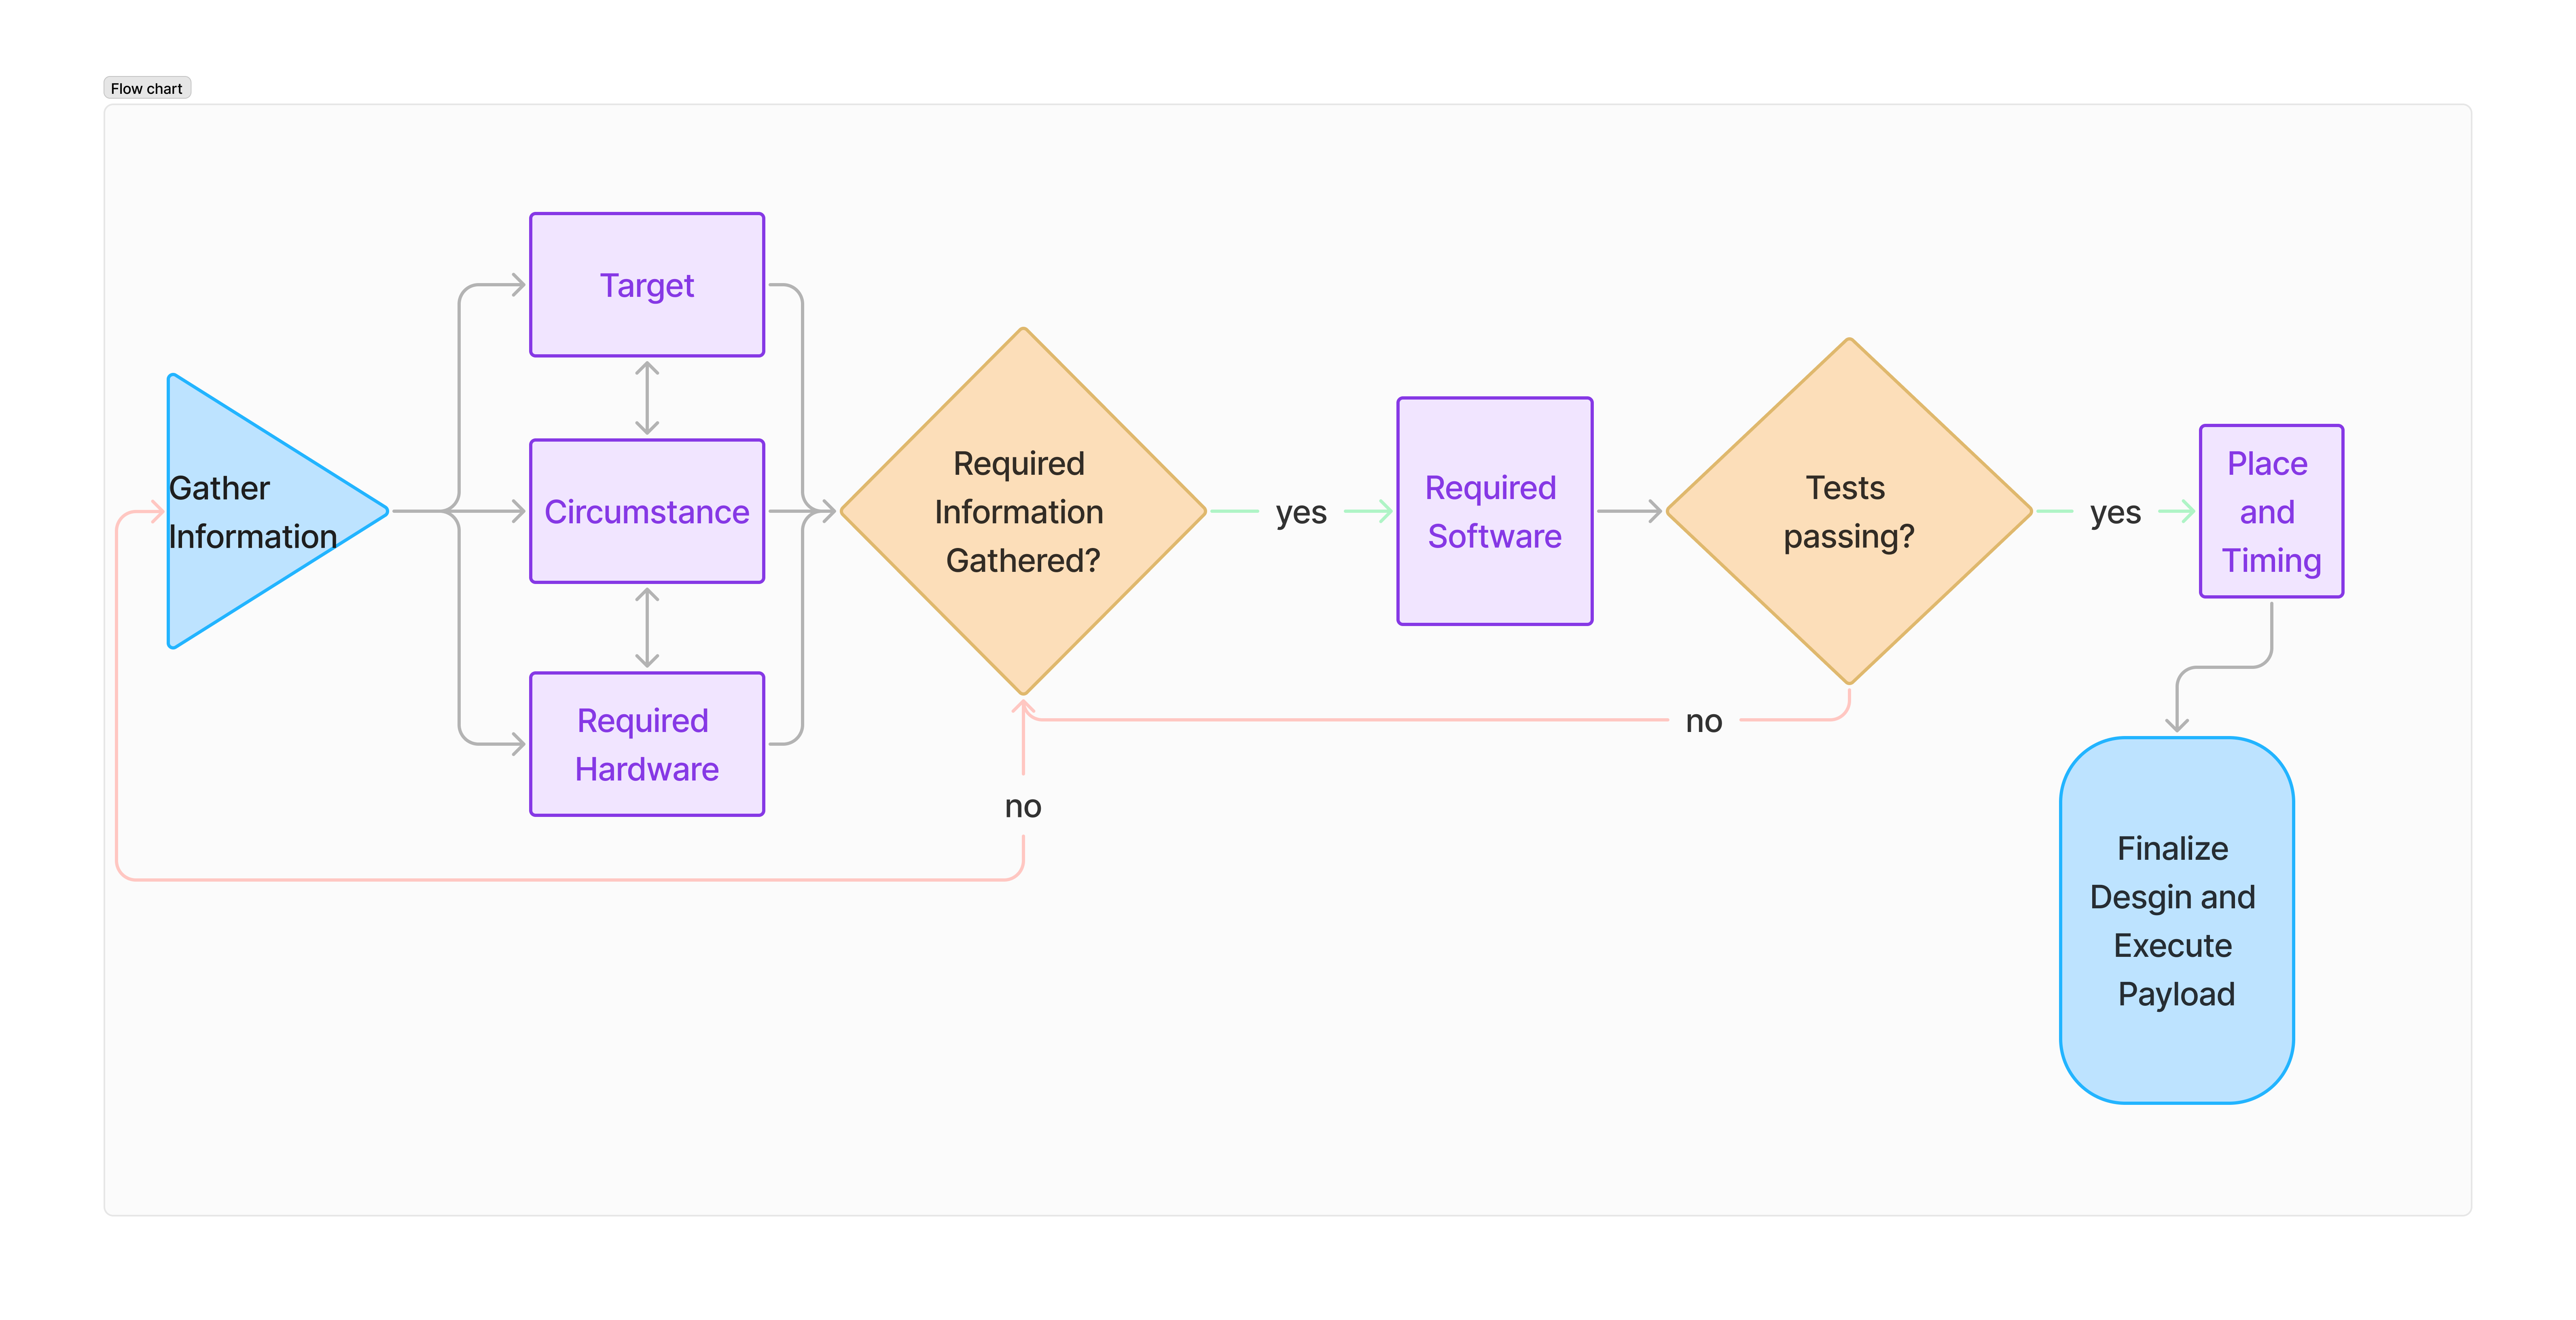
\includegraphics[width=1.1\linewidth]{visuals/Attack Development(1).png}
    \caption{Development process for a payload}
    \label{Flow Diagram Development process payload}
\end{figure}



\subsection{Command Line vs User Interface}

Payloads follow a combination of two main strategies; 
\begin{itemize}
    \item User Interface (UI) based
    \item Command Line Interface (CLI) based
\end{itemize}

UI-based payloads follow the line of action a typical UI-focused user would take. For example, for sending an email, such a user might search for the email application icon on their desktop, click on it, then click on 'new Mail', fill out all the fields of the email form, and finally click on send. A payload that mimics this behaviour, would navigate in the same way, using the keyboard instead of the mouse. For instance, if the Outlook icon was the fourth icon on the taskbar, it could be selected with the Windows key + 3. The 'new Mail' button would be reached with 16 tabs or by using  Ctrl + N. All navigation can be done in this manner and therefore programmed as an O.MG script. \\
Possible issues with this approach are obvious; How can you determine the location of Outlook on the taskbar? What if the computer is not connected to the Internet and instead of opening Outlook an error message pops up? What if the computer is very slow and  Ctrl + N is sent before the application has fully loaded?  Some of these issues can be accounted for, Outlook for instance can also be opened by searching for it in the start menu, however, determining whether the application has loaded is impossible with the O.MG cable. The risk can be mitigated by implementing long delays between commands. Unfortunately, this creates time overhead which can be a big drawback in time-sensitive situations. \\

A command-line-based approach eliminates such problems. It allows for a cleaner and more concise execution of an attack. It simplifies many actions and is often more direct and therefore faster. Take the mail example again. PowerShell has a cmdlet that allows you to send emails directly. This cuts down nearly all navigation and the risks and time overhead that come with it. \\
One drawback of this method is that it can more easily be identified as malicious activity. An average user would not use the command line to send an email let alone use it for anything else. Therefore actions like opening the Windows run window and starting powershell.exe can easily be flagged as suspicious behaviour. Another obstacle might be user privileges. Some commands require admin access, which is easy to deal with if the target is the admin user on the computer (simply deal with the popup) but requires the admin user's password if the target is not an administrator. 


\subsection{New Payloads}

This section provides an overview of the methodology for the newly developed payloads. Each payload is listed below along with its corresponding ATT\&CK category in parentheses:
\begin{enumerate}
    \item Register Email Forwarding (Collection)
    \item Disable Windows Event Logging (Defence Evasion)
    \item Extract SAM Hashes (Defence Evasion)
    \item Extract Private Key Files (Defence Evasion)
    \item Steal Web Session Cookies (Defence Evasion)
    \item Iteratively End Processes (Impact)
    \item Schedule Processes (Persistence)
\end{enumerate}


\begin{figure}[H]
    \centering
    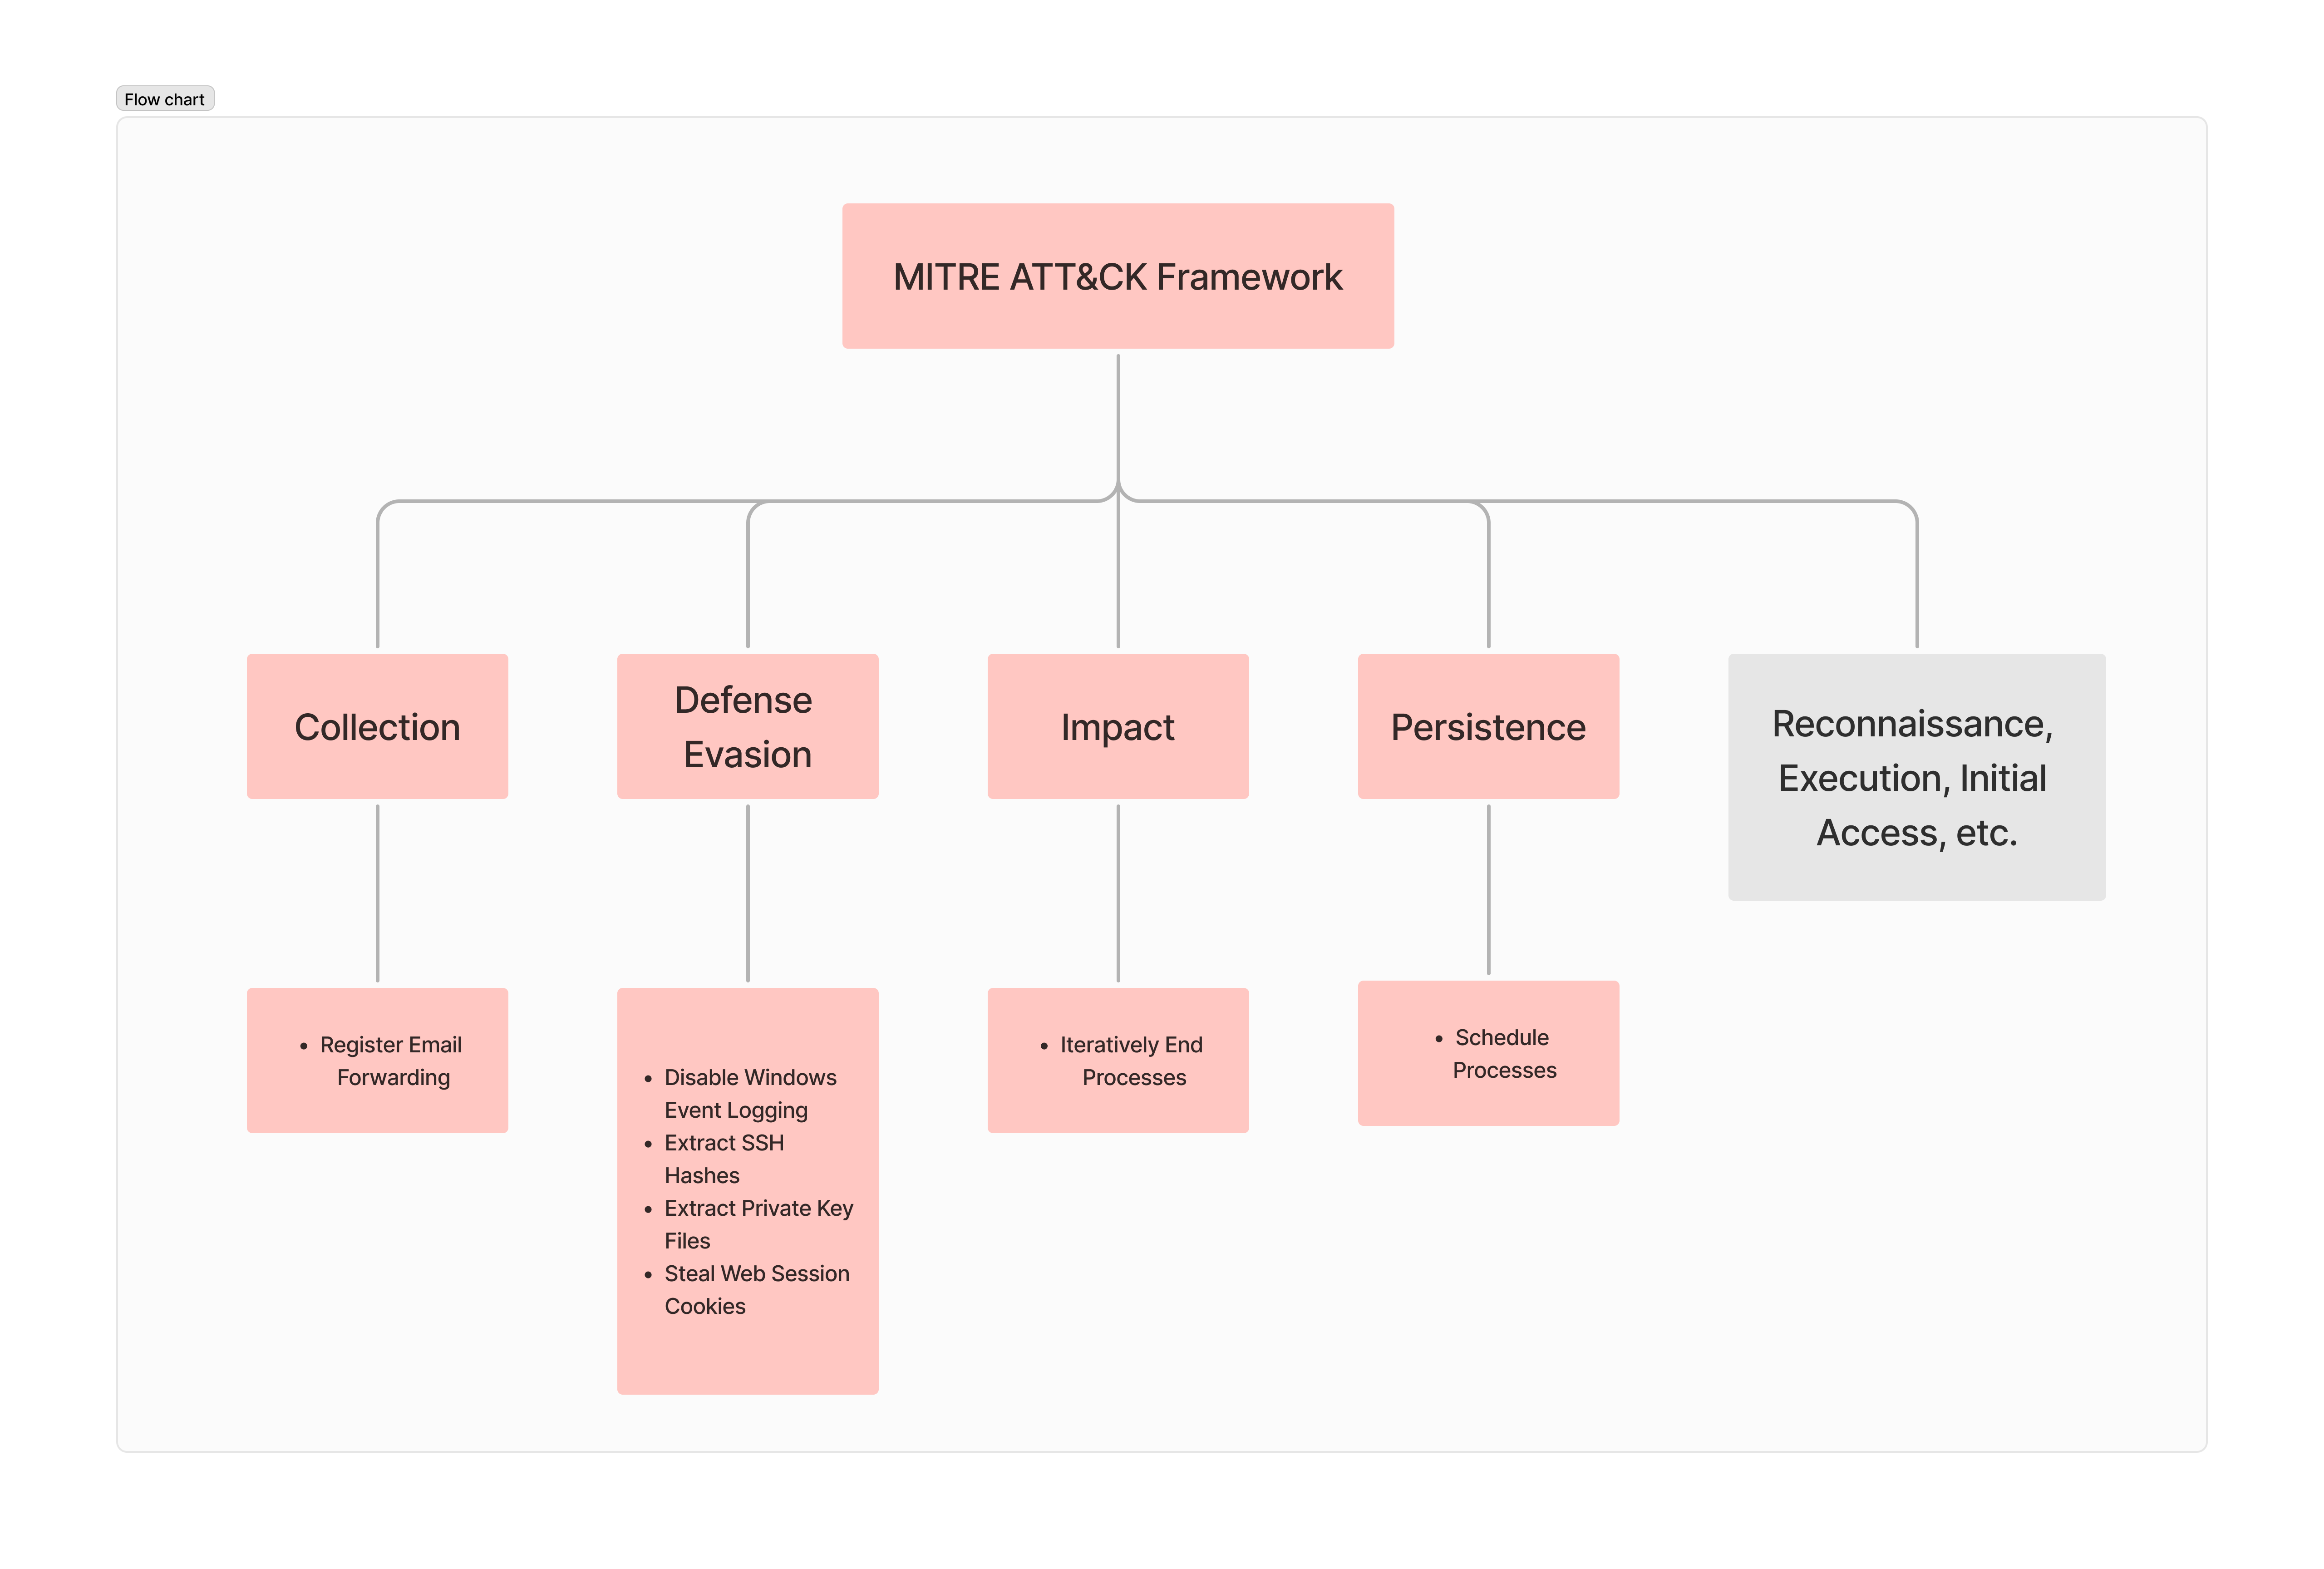
\includegraphics[width=1\linewidth]{visuals/payloads_overview.png}
    \caption{Overview over the featured payloads in terms of ATT\&CK categories}
\end{figure}





\subsubsection{Register Email Forwarding}

For reconnaissance purposes, it can be advantageous to monitor the emails a (potential) victim receives to observe personal and potentially sensitive information or to possibly obtain access to two-factor authentication codes, thereby facilitating unauthorized logins. One simple way to achieve this, which is not yet present in the official O.MG payload repository, is by registering email forwarding. 


\subsubsection{Disable Windows Event Logging}

Windows event logging is a built-in Windows functionality that logs the system's activity. There are multiple event types; Error, Warning, Information, Success Audit, and Failure Audit logged in multiple different categories; System Log, Application Log, Security, Setup and Forwarded Events. 
Some actions on a system might raise errors, warnings or other types of events in one of the logs, indicating that an attack has taken or is taking place. In order to avoid being found out during or after the attack, a hacker might attempt to disable the logging to leave as few traces as possible. For this reason, this kind of attack is classified under the ATT\&CK defence Evasion category. \\
There are multiple ways to disable Windows event logging, in the implementation chapter, a UI option and a CLI option will be presented. 


\subsubsection{Extract SAM hashes}

The Security Account Registry (SAM) on Windows stores user accounts and security descriptors \cite{archiveddocsSecurityAccountManager2009}, including, for example, passwords as hashes. These hashes can be exfiltrated and used to spoof the victim in a Pass the Hash attack. Passwords are often stored as hashes instead of cleartext, however, just like cleartext passwords, these hashes can be stolen and used to impersonate the user. This approach can also be used in the context of single sign-on systems to create new sign-on tickets using the stolen hash. This is used as a technique in the ATT\&CK lateral movement and Defence Evasion categories \cite{UseAlternateAuthentication}. \\
Access to these files is restricted to admin privileges on Windows, therefore this payload requires administrator privileges.

\subsubsection{Extract Private Key Files}

Public key cryptography builds on the notion of private and public keys that are calculated from a shared mathematical basis, such as the difficulty of factoring large prime numbers (in RSA \cite{rivestMethodObtainingDigital1978}). While it is extremely time and resource-consuming to try and reverse these calculations, a simpler way to breach this security mechanism is to steal the keys. Often, such private keys are stored in private key files that have corresponding file extensions and are stored in common file locations. Therefore, it is possible to search default directories for private key files for the mentioned file extensions and extract them.    


\subsubsection{Steal Web Session Cookies}

While most of the information stored in web session cookies might not be sensitive, it can always be used for reconnaissance and to learn about a target's habits and preferences which can help plan other attacks. However, the information can also include authentication tokens that are used as session cookies after a login \cite{StealWebSession}. The files in which this data is stored can be extracted from a client machine. \\
Such an attack first has to determine which browser should be targeted. For this, an attacker might search for the information of the default browser, send that information to a command server and then determine which extraction payload to trigger, based on that information. 


\subsubsection{Iteratively End Processes} \label{Iteratively End Processes}

One underexplored area of the MITRE ATT\&CK framework is the category 'Persistence'. This payload aims to achieve persistence by iteratively ending running processes. From all the running processes, the payload should stop those defined on a whitelist.


\subsubsection{Schedule Processes}

This payload aims to achieve persistence by registering processes that will run iteratively depending on a customizable trigger. These processes can be anything from reconnaissance scripts to other persistence payloads. This payload could for example be combined with the end processes payload in Section \ref{Iteratively End Processes} to create a payload that schedules the iterative termination of processes based on a predefined trigger.



\section{Defence Methodology} \label{Defence Methodology}

\subsection{Introduction}

To be able to defend against the existing and especially new threats introduced in this paper, this section will give an overview of the architecture for the announced defence script.

It has to be kept in mind, that most approaches are heuristics. Theoretically, it is always possible to circumvent them if enough resources are available. The only way to completely get rid of USB threats is to not use USB. In a closed system, all USB ports could be permanently blocked and the use of outside technology forbidden. As is often the case in cybersecurity, this is a matter of balancing usability and security. Restricting access and thereby usage of USB devices necessarily also diminishes or extinguishes the additional value they might bring. The framework in this paper consists of components that try to minimize the impact of usability. The framework should be a support and not an additional vice on the users to ensure that it is not circumvented because it is too tedious to work with.  

In order to be able to defend the payloads that were just introduced, the next section will outline a defence methodology.
This defence has two pillars:
\begin{enumerate}
    \item A classic rate limiter as seen in other papers (for example \cite{neunerUSBlockBlockingUSBBased2018} )
    \item Enumeration Packet Analysis
\end{enumerate}

Rate Limiting aims to catch the superhuman input speeds of O.MG cables (up to 890 keystrokes per second \cite{hak5MGCable}) while packet analysis is focused on monitoring the properties of connected devices for abnormalities.


\subsection{Traffic Capture} \label{Traffic Capture}

On Windows, USB packets can be captured with Wireshark, an application written to capture general web traffic \cite{WiresharkGoDeep}. It can be extended with 'USBPcap' \cite{USBPcap}, open-source software that allows the additional capture of USB packets in Wireshark. USBPcap can also be run via the command line separately from Wireshark, however, the visualization in the Wireshark application makes manual analysis easier. For visual analysis of USB frames, Bluetooth should be turned off since its packets are translated into USB and will therefore show up when using Wireshark with USBPcap. For automated analysis via the command line, Wireshark provides a command line application called Tshark \cite{TsharkTsharkDev}. 

For this capture, Wireshark 4.2.5-x64 in combination with USBPcap version 1.5.4.0 was used on a Windows Surface 4 Laptop with Windows Home version 23H2. Wireshark has to be run as administrator to make the capture of USB traffic possible.


\subsection{Packet Analysis}\label{Packet Analysis}


As inspired by other works that analyzed USB packets, for example, USBSafe \cite{kharrazUSBESAFEEndPointSolution2019} this paper seeks to find differences in USB Packets that were produced during the enumeration process of an O.MG cable versus those produced by unmodified external keyboards. In contrast, USBSafe focused on the timing, types and payloads of the packets throughout an entire interaction and did not specifically compare two types of USB devices, instead, they trained a model that distinguishes between known (safe) patterns in USB traffic and unknown (malicious) patterns. 

To this end, the following keyboards were examined:
\begin{enumerate}
    \item Ducky One 2 SF
    \item Sharkoon TODO what model exactly
    \item Glorious GMMK-TKL-RGB-ISO
\end{enumerate}


All USB communication is based on USB packets. As introduced in Section \ref{TheUSBProtocol} a newly connected USB device will first establish itself with the host via a process called enumeration, during which the device's capabilities and services are communicated to the host. Once the device has completed enumeration following the USB protocol, it is ready for use.
All information transferred during and after this process, is packaged in USB packets, also called USB frames. The frames are then interpreted by the OS to determine their meaning and the commands they contain.



\subsubsection{Basics of Packet Analysis}

The frames exchanged during the enumeration process contain information about the connected device, which is especially valuable for identifying its USB class and protocols.
Packets such as Device Descriptors and Interface Descriptors allow concluding a device's functionality. Take for example the frame in Listing \ref{lst:example_frame_bluetooth}:

\begin{lstlisting}[caption={Device Descriptor packet of a wireless controller}, label={lst:example_frame_bluetooth}, captionpos=b]
Frame 8: 46 bytes on wire (368 bits), 46 bytes captured (368 bits) on interface \\.\USBPcap2, id 1
USB URB
    [Source: 2.2.0]
    [Destination: host]
    USBPcap pseudoheader length: 28
    IRP ID: 0x0000000000000000
    IRP USBD_STATUS: USBD_STATUS_SUCCESS (0x00000000)
    URB Function: URB_FUNCTION_CONTROL_TRANSFER (0x0008)
    IRP information: 0x01, Direction: PDO -> FDO
        0000 000. = Reserved: 0x00
        .... ...1 = Direction: PDO -> FDO (0x1)
    URB bus id: 2
    Device address: 2
    Endpoint: 0x80, Direction: IN
        1... .... = Direction: IN (1)
        .... 0000 = Endpoint number: 0
    URB transfer type: URB_CONTROL (0x02)
    Packet Data Length: 18
    [Request in: 7]
    [Time from request: 0.000000000 seconds]
    Control transfer stage: Complete (3)
DEVICE DESCRIPTOR
    bLength: 18
    bDescriptorType: 0x01 (DEVICE)
    bcdUSB: 0x0201
    bDeviceClass: Wireless Controller (0xe0)
    bDeviceSubClass: 1
    bDeviceProtocol: 1 (Bluetooth Programming Interface)
    bMaxPacketSize0: 64
    idVendor: Intel Corp. (0x8087)
    idProduct: AX201 Bluetooth (0x0026)
    bcdDevice: 0x0002
    iManufacturer: 0
    iProduct: 0
    iSerialNumber: 0
    bNumConfigurations: 1
\end{lstlisting}

The first section of the frame contains meta information, such as the status, the function, length of the pseudo-header. The second section contains the actual information that is transferred.
This is a device descriptor packet that communicates to the host what kind of device it is. In this case, it is a wireless controller that applies the Bluetooth programming interface. It also specifies the
vendor and product IDs. Some information such as the manufacturer, product and serial number are left blank here.
This source device is a built-in Bluetooth adapter that translates Bluetooth traffic into USB. It illustrates one of the challenges of packet analysis; filtering out noise in traffic. If one were to capture USB traffic while the host is connected to a Bluetooth
speaker, for example, there would be constant traffic generated from streaming music. This traffic should not be considered for rate limiting since it is automatically generated and required to be fast.
For this reason, extracting information such as the device classes and protocols is important. A Device Descriptor for a keyboard is shown in Listing \ref{lst:device_descriptor_frame} below. 


\begin{lstlisting}[caption={Device Descriptor packet generated by an external keyboard},label={lst:device_descriptor_frame}, captionpos=b]
DEVICE DESCRIPTOR
    bLength: 18
    bDescriptorType: 0x01 (DEVICE)
    bcdUSB: 0x0200
    bDeviceClass: Device (0x00)
    bDeviceSubClass: 0
    bDeviceProtocol: 0 (Use class code info from Interface Descriptors)
    bMaxPacketSize0: 64
    idVendor: Unknown (0x320f)
    idProduct: Unknown (0x5016)
    bcdDevice: 0x0119
    iManufacturer: 1
    iProduct: 2
    iSerialNumber: 0
    bNumConfigurations: 1
\end{lstlisting}


This is a device descriptor from a Sharkoon Keyboard. It does not carry keyboard-specific information but rather describes the device as generically as possible. This is not always the case, for example, the Glorious GMMK keyboard carries the line: \verb|idProduct: Backlit Gaming Keyboard (0x652f)|. Nevertheless,
it means that the Device Descriptor packets alone are not enough to determine what device the host is dealing with. This is where the Interface Descriptor packets come into play, one of them is shown in Listing \ref{lst:interface_descriptor_frame}.
This is the Interface Descriptor for the Sharkoon keyboard whose generic Device Descriptor was presented in Listing \ref{lst:device_descriptor_frame}.

\begin{lstlisting}[caption={Interface Descriptor packet generated by an external keyboard}, label={lst:interface_descriptor_frame}, captionpos=b]
INTERFACE DESCRIPTOR (0.0): class HID
    bLength: 9
    bDescriptorType: 0x04 (INTERFACE)
    bInterfaceNumber: 0
    bAlternateSetting: 0
    bNumEndpoints: 1
    bInterfaceClass: HID (0x03)
    bInterfaceSubClass: Boot Interface (0x01)
    bInterfaceProtocol: Keyboard (0x01)
    iInterface: 0
\end{lstlisting}

It specifically describes the device as a Human Interface Device (HID) and the interface protocol as ``Keyboard'' with the corresponding hexadecimal HID code for a keyboard; ``0x01''.

Device Descriptor and interface packets describe the function of a USB device and identify it as a keyboard to the host. In order to spoof a keyboard, an O.MG cable would have to do the same. So what do these packets look like for an O.MG cable?
First off, it is important to note that the cable is not enumerated as a keyboard immediately after being plugged in. When first inserted into a host, no communication happens, since it is acting as a simple cable which does not require communication with the host. However, every time a payload is executed, the cable enumerates as a keyboard.
Listing \ref{lst:device_and_interface_frame_OMG} shows these Device Descriptor and Interface packets;

\begin{lstlisting}[caption={Device and Interface Descriptor packet generated by an O.MG cable}, label={lst:device_and_interface_frame_OMG} , captionpos=b]
DEVICE DESCRIPTOR
    bLength: 18
    bDescriptorType: 0x01 (DEVICE)
    bcdUSB: 0x0110
    bDeviceClass: Device (0x00)
    bDeviceSubClass: 0
    bDeviceProtocol: 0 (Use class code info from Interface Descriptors)
    bMaxPacketSize0: 8
    idVendor: Unknown (0xd3c0)
    idProduct: Unknown (0xd34d)
    bcdDevice: 0x0002
    iManufacturer: 1
    iProduct: 2
    iSerialNumber: 3
    bNumConfigurations: 1


INTERFACE DESCRIPTOR (1.0): class HID
    bLength: 9
    bDescriptorType: 0x04 (INTERFACE)
    bInterfaceNumber: 1
    bAlternateSetting: 0
    bNumEndpoints: 1
    bInterfaceClass: HID (0x03)
    bInterfaceSubClass: Boot Interface (0x01)
    bInterfaceProtocol: Keyboard (0x01)
    iInterface: 0
\end{lstlisting}

As we can see, there are no relevant differences between the packets from the Sharkoon keyboard compared to the O.MG cable besides some technical differences such as their maximum packet size or their release numbers in binary-coded decimal (bcdUSB). This raises the question of whether the O.MG cable is distinguishable
from a non-malicious keyboard through its USB traffic. In theory, it does not have to be; to the host, it acts like any other keyboard in every regard with the same functionality. There are no obvious differences. In the following, this paper analyses the USB traffic in more detail to find out if this is the case.


\subsubsection{Remote Wakeup}

Early in the enumeration, packet 16, the first big difference can be found: While all three external keyboards describe themselves to have the attribute 'REMOTE-WAKEUP' the O.MG cable specifies in this packet that it has 'NO REMOTE WAKEUP'. This difference can be seen in Figure \ref{fig:packet16OMG} vs \ref{fig:packet16Ducky}. Keyboards with 'REMOTE WAKEUP' can send a signal to a 'sleeping' host that can wake it. This is common for HIDs and can also be seen in mice that can be moved to wake a host. The O.MG cable, however, does not have that capability. When a payload is executed while the target is asleep, it is not woken up and therefore the input is not processed. This is a weird anomaly. A HID device, specifically a keyboard, should be able to wake the host. How else, would a desktop without built-in HID devices be woken up? An HID device without this functionality does not provide a basic feature of human-computer interaction and is therefore suspicious.

\begin{figure}[H]
    \centering
    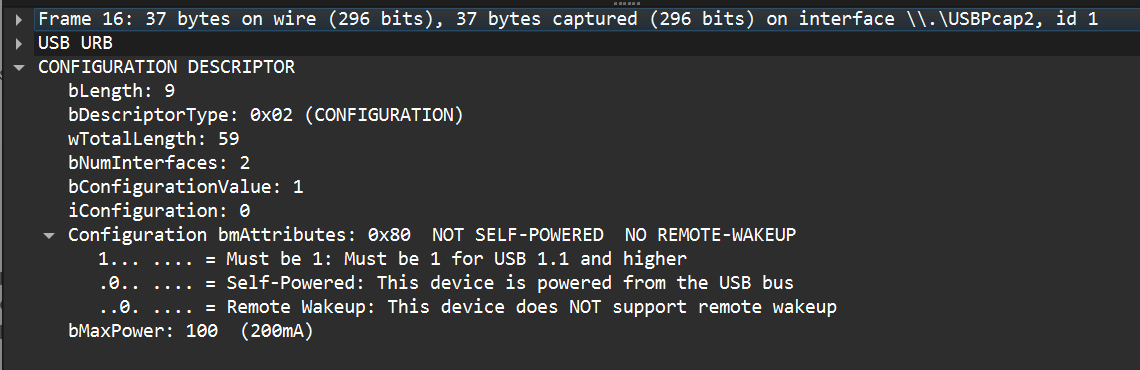
\includegraphics[width=0.75\linewidth]{visuals/no-remote-wakeup-100mA.png}
    \caption{Packet no. 16 of an O.MG Cable enumeration}
    \label{fig:packet16OMG}
\end{figure}

\subsubsection{Technical Data}

Just like the REMOTE WAKEUP property, the amount of power a non-self-powered device requires is specified within the first packets. There is difference that can be observed between the Ducky keyboard and the rest of the devices. While 3 of the 4 devices specify 'bMaxPower' in packet 15 to be "100 (200mA)" (figure \ref{fig:packet16OMG}, the Ducky's current consumption is "50 (100mA)" as seen in Figure \ref{fig:packet16Ducky}. Maximum current consumption can therefore not be used as an indicator for the presence of an O.MG cable since it varies within the keyboard class as well. 


\begin{figure}[H]
    \centering
    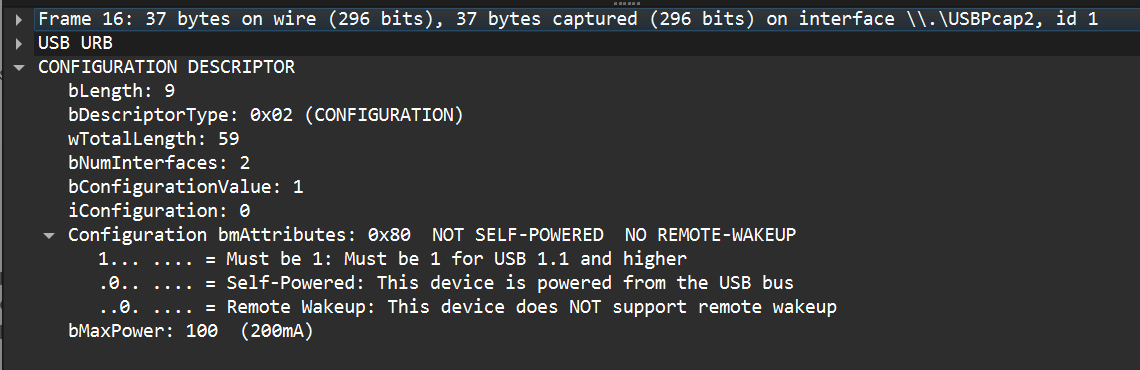
\includegraphics[width=0.75\linewidth]{visuals/no-remote-wakeup-100mA.png}
    \caption{Packet no. 16 of a Ducky Keyboard enumeration}
    \label{fig:packet16Ducky}
\end{figure}


\subsubsection{Register as multiple devices}

All the devices register as multiple HID devices corresponding to their device functions as explained in Chapter \ref{Background}. The Sharkoon and Glorious keyboards first register as a keyboard, then as a mouse. The Ducky registers as keyboard first and as multiple different ``HID Report''s later. The O.MG cable is the only one that registers as a mouse first and as a keyboard second. This can be seen in packet 18 for all the devices; figure \ref{fig:packet18Glorious} shows an example of the Glorious Keyboard specifying the enumeration as keyboard and mouse. 

\begin{figure}[H]
    \centering
    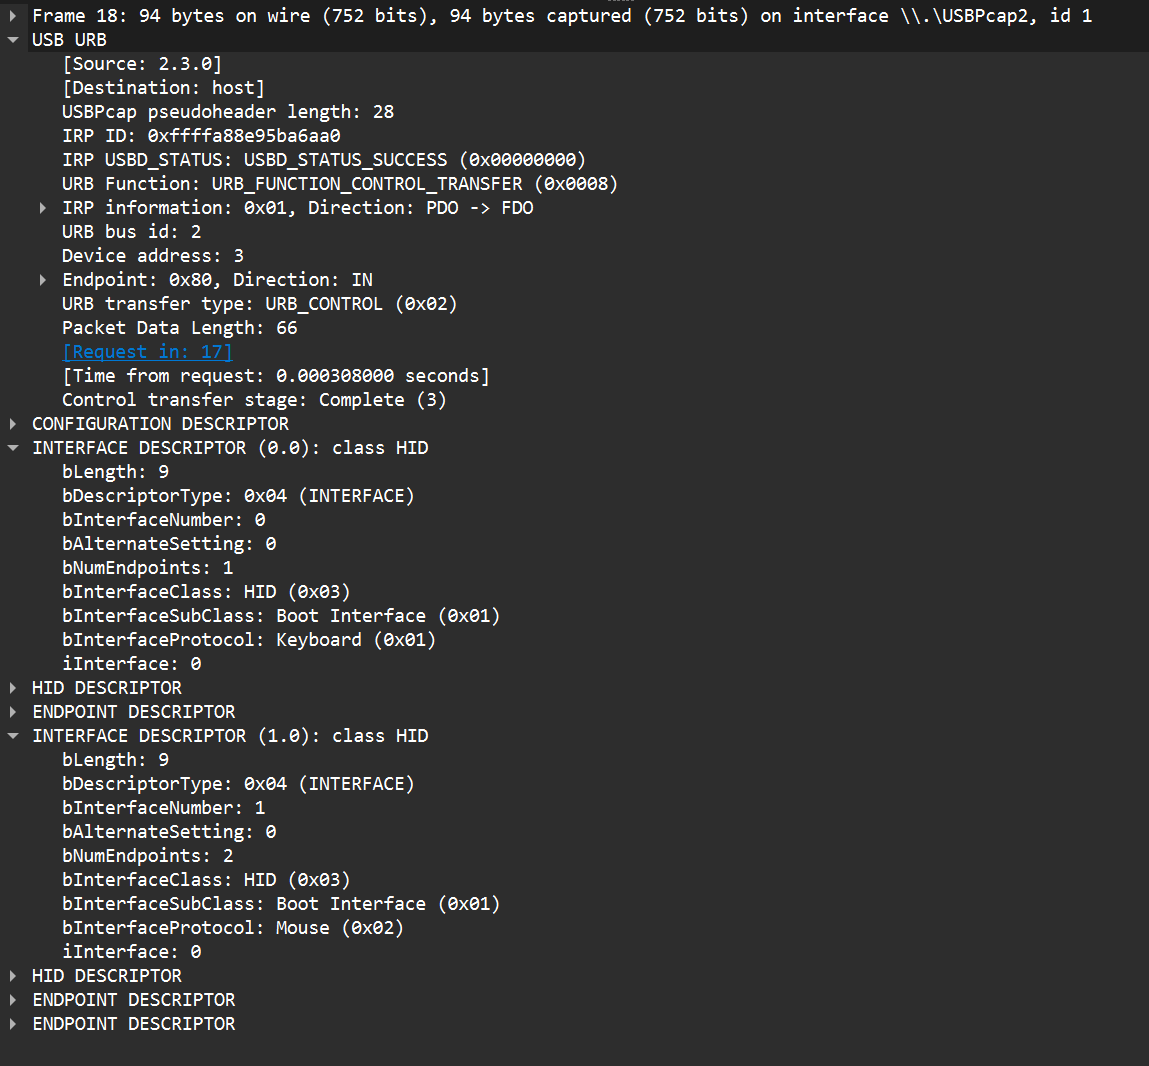
\includegraphics[width=0.75\linewidth]{visuals/packet18glorious.png}
    \caption{Packet no. 18 of a Glorious Keyboard enumeration}
    \label{fig:packet18Glorious}
\end{figure}

\subsubsection{Length of Descriptors}

In various instances, the devices differ in their metadata. For example in packet 26 of the Sharkoon keyboard the bLength descriptor is 46, while for the Ducky it is 36, the Glorious 22 and the O.MG 10. Similarly, the number for wLength differs in packet 27. These descriptors vary every time they occur and between all the devices. Therefore, they cannot be used as a differentiator between malicious and harmless devices. Furthermore, since the lengths of the descriptors depend on the descriptors themselves, and the O.MG descriptors can easily be changed, this is not a reliable metric.
This also explains the differences in the bString itself, for example in packet 28, where the manufacturer's name is spelled out. Just as with the descriptors, any manufacturer can easily be spoofed by an O.MG cable by changing its settings. 


\subsubsection{Unrecognized Packets}

All external keyboards have packet exchanges that Wireshark flags as 'Unknown type' which seems to be some Wireshark error for reading and interpreting the packets. The issue seems to have to do with the descriptors request that are specific for Windows \cite{USBPcapDidNot}.

\begin{figure}[H]
    \centering
    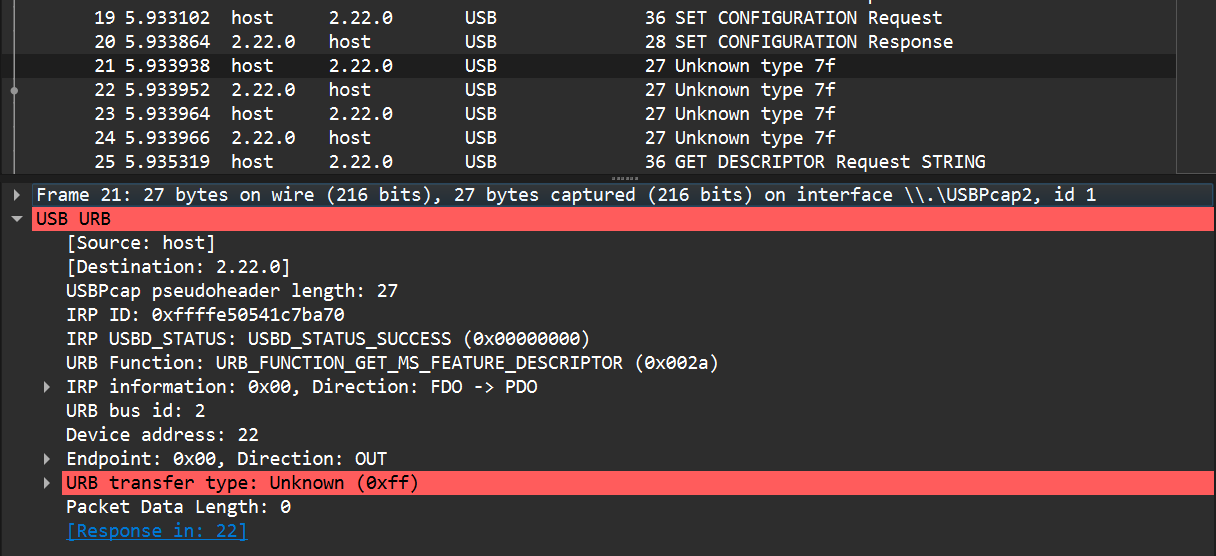
\includegraphics[width=0.75\linewidth]{visuals/unknownPacketsSharkoon.png}
    \caption{Unknown type Packets as an example from the Sharkoon enumeration}
    \label{fig:unknownPacketsSharkoon}
\end{figure}


\subsubsection{Larger Differences in Packet Types, Number and Order}

Due to some unrecognized packets and differences in enumeration order and the number and device functions that are enumerated, the packets start to lose their alignment with each other around packet 30. From thereon, they are hard to compare directly. Some devices have more unrecognized packets, some different numbers of 'collection', 'usage page', 'usage', 'set\_report', and 'descriptor' packets. However, there seem to be no discernable patterns for this reason and the differences also occur within the external keyboard group. Judging by this small sample size, the O.MG has the smallest number of packets exchanged for enumeration. 


\subsubsection{Conclusion Packet Analysis}

The biggest difference in the enumeration phase of these devices is in the number and type of packets, however, they still follow the same pattern, given by the USB protocol. More reliable patterns might be found with a much bigger sample size and statistical analysis. This is out of scope for this thesis but should be considered in future works. (TODO; add this to limitations). Generally speaking, the cable seems to be more efficient than the external keyboards while enumerating using the least amount of packets overall.
Differences in descriptors, lengths and other metadata (like technical specifications) are non-conclusive for distinguishing the O.MG cable. 
The most apparent and striking difference is that the O.MG cable is enumerated with the 'NO REMOTE WAKEUP' attribute, which sets it apart from all other keyboards.
A defence system based on qualitative packet analysis can be built on this difference. It requires tracking the enumeration of all USB devices that enumerate as keyboards and checking for their remote wakeup attribute. 

It is not surprising that the enumeration of the O.MG cable does not differ more extremely from that of usual external keyboards. For the host, it looks like any other keyboard and functions like one too. Enumeration is therefore also the same. Additionally, the possible differences are restricted because of the established USB protocol.

It is important to note that while this thesis can only conclude the presence of one clear factor that points to the presence of an O.MG cable, it does not mean that more do not exist. Possible patterns could be found with a scientific experiment featuring a big and statistically significant number of external keyboards (100+) and multiple O.MG cables.

\subsection{Rate Limiting}

A second use of monitoring USB traffic is rate limiting. In addition to the qualitative analysis of enumeration traffic, this quantitative approach detects anomalies in keyboard input. O.MG cables can generate keystrokes at superhuman speeds; 890 keystrokes per second (keys/sec) for the elite version and 120 keystrokes per second for the basic version. Currently, what is considered elite human typing are speeds around 200 to 300 words per minute \cite{mythicalrocketTYPING305WPM2023}. Words per minute are calculated as the number of typed characters divided by 5 \cite{travisWhatWordsMinute2015}. 300 words per minute would therefore be 300x5 / 60 = 25 keystrokes per second, about a fifth of what a basic O.MG cable can achieve.
Keystrokes this fast are suspicious and indicate non-human input. A rate limiter should monitor all keyboard input and their speed. Once inputs surpass a threshold, the user should be alarmed and the device disconnected to stop the attack. \\
The challenge in the design of such a rate limiter is the threshold. What should the threshold effectively be? A measurement like this requires a time window in which it is measured. The greater the amount of available data, which implies a longer measurement window, the more accurate the conclusion. However, this means more time for executing an attack; if the cable can input 120 keystrokes per second and a rate limiter has a window of one second, all payloads under 120 keystrokes are theoretically able to circumvent the defence mechanism. In practice, these payloads would also need to introduce delays, pushing their total execution time beyond one second.
Such delays would, however, also enable payloads longer than 120 keystrokes. To illustrate, pressing Windows Key + R opens the Run window, followed by a brief pause to allow the host to respond, before entering 'PowerShell' and pressing Enter. Assuming that the input + wait time would take one second, that is an input speed of 12 keys/sec half the speed of attainable human input. Simply delaying a payload after every 10 keystrokes circumvents a rate limiter that checks one-second intervals.\\
Another possible approach is measuring the input time between individual keystrokes, which might become a problem for key combinations, gaming and spamming keys manually. 25 keystrokes per second comes out to a limit of 40 milliseconds interarrival time between keys for human input. All interarrival times below this threshold ought to be considered machine-generated. Similarly to the time window approach, this value could also be calculated as an average over a number of keystrokes. To circumvent it, many small delays are necessary between the individual keystrokes.\\
Either method can be circumvented with delays, however, they can still be useful for catching less intricate attacks that are unprepared against rate limiting.
Chapter \ref{Implementation} will explain how both approaches can be realized and their results will be discussed in chapter \ref{Evaluation}.


To measure these speeds, the defence framework has to store the times at which HID input packets arrive for a specific keyboard. These packets have to be mapped to their sources, to ensure that the program knows which USB device it has to disconnect to stop the attack. This means this type of monitoring must be linked to packet analysis to avoid false triggers from mouse or Bluetooth traffic.

Figure \ref{fig:defence_flowchart} visualizes the defence process as a flow chart, starting with the enumeration pattern detection and moving on to the two different rate limiter modes. 

\begin{figure}[H]
    \centering
    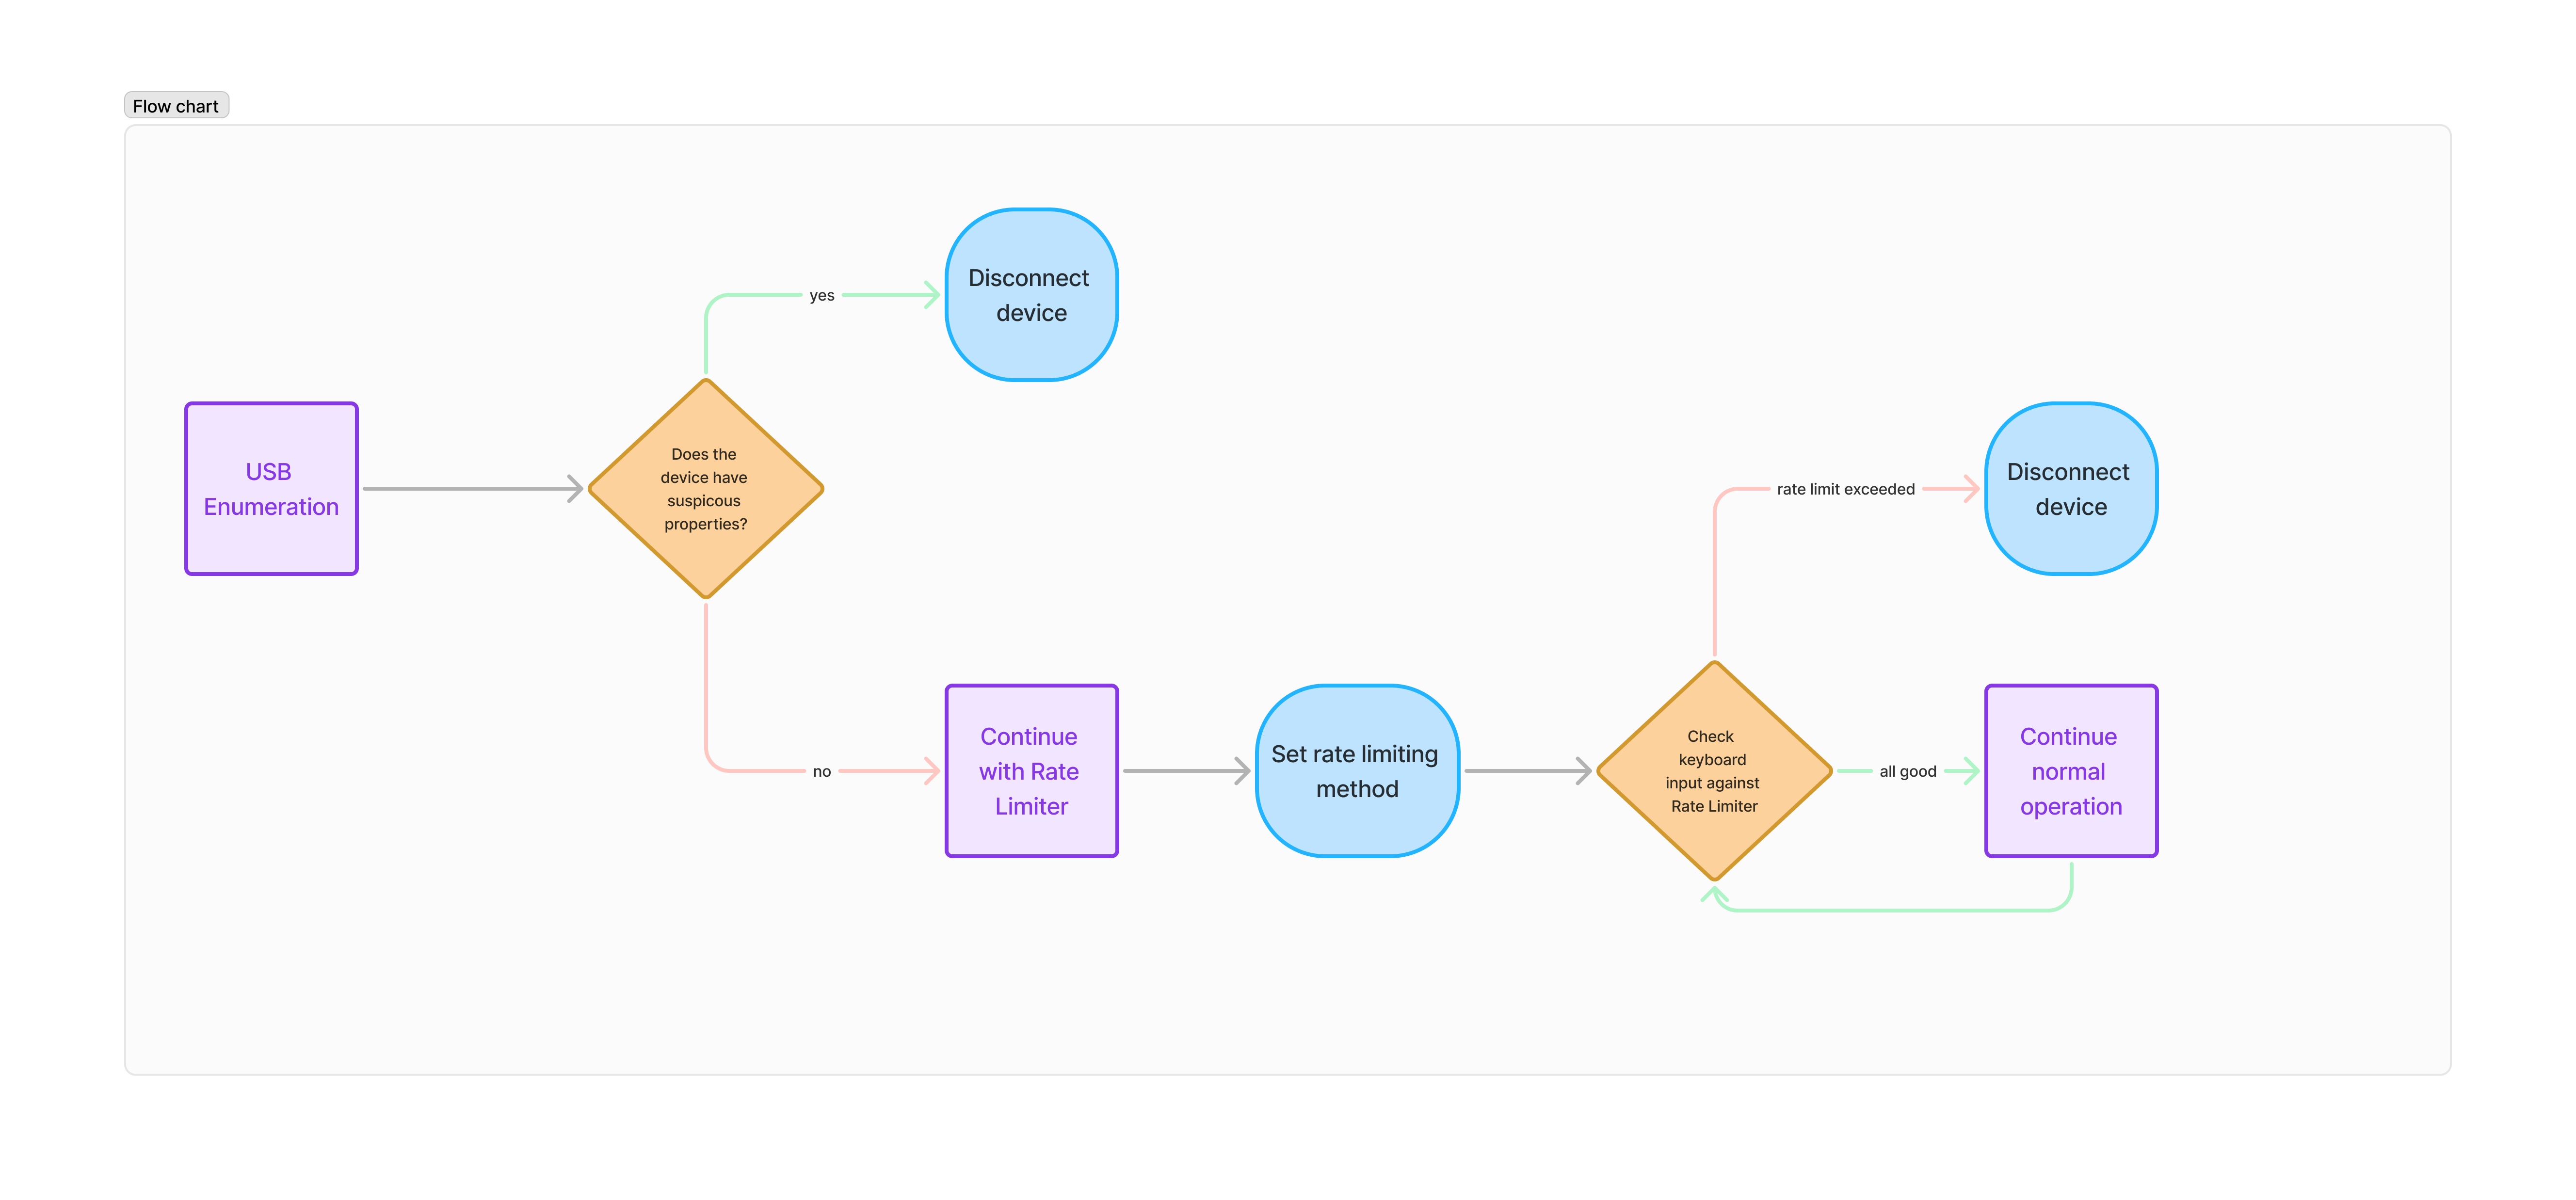
\includegraphics[width=1\linewidth]{visuals/defense_flowchart.png}
    \caption{Flowchart describing the Defence Architecture}
    \label{fig:defence_flowchart}
\end{figure}


\section{Conclusion Methodology and Architecture}

This chapter introduced the underlying architecture and methodology for both the attack side through the newly developed payloads as well as the defence by introducing the developed defence system and its components. 
It started by introducing the MITRE ATT\&CK framework and some of its 14 categories. Then, it mapped the payloads from the official open-source O.MG payloads repository on GitHub onto those categories to find out which techniques were already present and available and which ones were underrepresented or missing completely. After that, it introduced the architecture of a few payloads that would fill some of those gaps using techniques that had not yet been featured in the source code. \\
In a second section of the chapter, the thesis outlined a defence framework that featured qualitative and quantitative packet analysis, monitoring traffic for a specific enumeration signature of O.MG cables and the speed at which HID input packets are received. Next this thesis will explain how the approaches introduced in this chapter can be applied and implemented for real-world usage. 



